\section{Introducción:}

\subsection{subsecci\'on}
  \begin{enumerate}
    \item Algo
    \item Algo
  \end{enumerate}
\subsection{secci\'on}
  \begin{lstlisting}[language=Python]
    import socket

    UDP_IP = "127.0.0.1"
    UDP_PORT = 5005
    MESSAGE = "Hello, World!"

    print "UDP target IP:", UDP_IP
    print "UDP target port:", UDP_PORT
    print "message:", MESSAGE

    sock = socket.socket(socket.AF_INET, # Internet
                          socket.SOCK_DGRAM) # UDP
    sock.sendto(MESSAGE, (UDP_IP, UDP_PORT))
  \end{lstlisting}
\subsection{subsecci\'on}
  %Eliminar la sangría al comienzo de un párrafo
  \noindent
  Esta es una cita \cite{einstein}\\
  Esta es otra cita \cite{dirac}\\
  Esta es otra cita \cite{knuthwebsite}\\
\subsection{subsecci\'on}
  \noindent
  \url{www.google.com.ar}
\subsection{subsecci\'on}
pie de p\'agina\footnote{info}
\begin{center}
    \begin{tabular}{ | l | l | l | p{5cm} |}
    \hline
    Day & Min Temp & Max Temp & Summary \\ \hline
    Monday & 11C & 22C & A clear day with lots of sunshine.
    However, the strong breeze will bring down the temperatures. \\ \hline
    Tuesday & 9C & 19C & Cloudy with rain, across many northern regions. Clear spells
    across most of Scotland and Northern Ireland,
    but rain reaching the far northwest. \\ \hline
    Wednesday & 10C & 21C & Rain will still linger for the morning.
    Conditions will improve by early afternoon and continue
    throughout the evening. \\
    \hline
    \end{tabular}
\end{center}

\begin{center}
\begin{tabular}{|c|c|c|}
  \hline
  \textbf{asd}     & \textbf{asd} & \textbf{asd}\\\hline\hline
      &			     			  & 123 \\ \cline{3-3}
  dsa& \multirow{-2}{*}{as} & 123\\ \hline
      &			                  & 123 \\ \cline{3-3}
  dsa& \multirow{-2}{*}{as} & 123\\ \hline
              &			& 123\\ \cline{3-3}
                & \multirow{-2}{*}{as} & 123\\ \cline{2-2}\cline{3-3}
               & 			&123\\ \cline{3-3}
  \multirow{-4}{*}{dsa} & \multirow{-2}{*}{as} & 123\\\hline
\end{tabular}
\end{center}

\begin{center}
	\begin{tabular}{ |l|l|l| }
		\hline
		\multicolumn{3}{ |c| }{Team sheet} \\
		\hline
		Goalkeeper & GK & Paul Robinson \\ \hline
		\multirow{4}{*}{Defenders} & LB & Lucas Radebe \\
		& DC & Michael Duburry \\
		& DC & Dominic Matteo \\
		& RB & Didier Domi \\ \hline
		\multirow{3}{*}{Midfielders} & MC & David Batty \\
		& MC & Eirik Bakke \\
		& MC & Jody Morris \\ \hline
		Forward & FW & Jamie McMaster \\ \hline
		\multirow{2}{*}{Strikers} & ST & Alan Smith \\
		& ST & Mark Viduka \\
		\hline
	\end{tabular}
\end{center}

%Ejemplo donde se ajusta el tamaño de la tabla con resizebox
\begin{center}
	\resizebox{\textwidth}{!}{%
	\begin{tabular}{ |l|l|l|l|l|}
		\hline
		\multicolumn{5}{ |c| }{\textbf{Tabla 1 - L\'ineas de Balmer del H}} \\
		\hline\hline
		Nro & $\lambda_1 = x_1 \pm \Delta x_1$ & $\lambda_2 = x_2 \pm \Delta x_2$ &$\lambda_3 = x_3 \pm \Delta x_3$ & $\lambda_3 = x_3 \pm \Delta x_3$\\ \hline
		1 &  & & &\\ \hline
		2 &  & & &\\ \hline
		3 &  & & &\\ \hline
		4 &  & & &\\ \hline
		5 &  & & &\\ \hline
		Resultado & $<x_1>\pm E_{x_1}$ &  $<x_2>\pm E_{x_2}$  & $<x_3>\pm E_{x_3}$ & $<x_4>\pm E_{x_4}$\\
		\hline
	\end{tabular}}
\end{center}

%\mc es la definición del comando el número entre corchetes especifica la cantidad de argumentos y el #1 indica el lugar del primer argumento.
\newcommand{\mc}[1]{\multicolumn{1}{c}{#1}}

%Poner dos tablas rotadas una debajo de la otra
\begin{table}[!htb]
\rotatebox{90}{
\begin{minipage}{.50\linewidth}
		\caption{Tabla 1}
		\begin{tabular}{c|c|c|c|c|c|}
		\mc{} & \mc{A} & \mc{B} & \mc{C} &  \mc{D} & \mc{E} \tabularnewline \hhline{~|*{5}{-}}
		a           						 &  \cellcolor{blue!25}        &                                        &                                          &                                          &  \cellcolor{red!25}   \tabularnewline \hhline{~|*5-}
		b          							 &                                          &                                       &                                           &                                          &  \tabularnewline \hhline{~|*5-}
		c           						 &                                          &                                        &                                          &                                         &  \tabularnewline \hhline{~|*5-}
		d           						 &                                          &                                        &                                         &                                          &  \tabularnewline \hhline{~|*5-}
		e           						 &                                          & \cellcolor{green!25}     &                                         &                                           &  \tabularnewline \hhline{~|*5-}
	\end{tabular}
\end{minipage}}
\rotatebox{90}{
\begin{minipage}{.50\linewidth}
	\caption{tabla 2}
	\begin{tabular}{c|c|c|c|c|c|}
		\mc{} & \mc{A} & \mc{B} & \mc{C} &  \mc{D} & \mc{E} \tabularnewline \hhline{~|*{5}{-}}
		a           						 &  \cellcolor{blue!25}        &                                        &                                          &                                          &  \cellcolor{red!25}   \tabularnewline \hhline{~|*5-}
		b          							 &                                          &                                       &                                           &                                          &  \tabularnewline \hhline{~|*5-}
		c           						 &                                          &                                        &                                          &                                         &  \tabularnewline \hhline{~|*5-}
		d           						 &                                          &                                        &                                         &                                          &  \tabularnewline \hhline{~|*5-}
		e           						 &                                          & \cellcolor{green!25}     &                                         &                                           &  \tabularnewline \hhline{~|*5-}
	\end{tabular}
\end{minipage}}
\end{table}

%Varias tablas a 90º vspace necesario para que las tablas no se superpongan con el título. "\\\\" después de end{tabular} para separar las tablas. newcolumntype permite dejar todas las celdas del mismo tamaño. 
\section{Ejercicio N\textdegree 1:}
\vspace{4.8cm}
\newcolumntype{C}{>{\centering\arraybackslash}p{1em}}
\begin{table}[H]
	\rotatebox{90}{
		\begin{minipage}{\linewidth}
			\subsubsection{1}
			\begin{tabular}{*{21}{C|}}
				\mc{0} & \mc{} & \mc{} & \mc{} &  \mc{} & \mc{5} & \mc{} & \mc{} & \mc{} &  \mc{} & \mc{10} & \mc{} & \mc{} & \mc{} &  \mc{} & \mc{15} & \mc{} & \mc{} & \mc{} &  \mc{} & \mc{20} \tabularnewline \hhline{~|*{20}{-}}
				A   & & & &  &  & & & & & & & & &  & & & & & &  \tabularnewline \hhline{~|*{20} -}
				B   & & & &  &  & & & & & & & & &  & & & & & &  \tabularnewline \hhline{~|*{20}-}
				C   & & & &  &  & & & & & & & & &  & & & & & &  \tabularnewline \hhline{~|*{20}-}
				D   & & & &  &  & & & & & & & & &  & & & & & &  \tabularnewline \hhline{~|*{20}-}
				E  & & & &  &  & & & & & & & & &  & & & & & &  \tabularnewline \hhline{~|*{20}-}
			\end{tabular}\\\\
	\end{minipage}}
	\rotatebox{90}{
		\begin{minipage}{\linewidth}
			\subsubsection{2}
			\begin{tabular}{*{21}{C|}}
				\mc{0} & \mc{} & \mc{} & \mc{} &  \mc{} & \mc{5} & \mc{} & \mc{} & \mc{} &  \mc{} & \mc{10} & \mc{} & \mc{} & \mc{} &  \mc{} & \mc{15} & \mc{} & \mc{} & \mc{} &  \mc{} & \mc{20} \tabularnewline \hhline{~|*{20}{-}}
				A   & & & &  &  & & & & & & & & &  & & & & & &  \tabularnewline \hhline{~|*{20} -}
				B   & & & &  &  & & & & & & & & &  & & & & & &  \tabularnewline \hhline{~|*{20}-}
				C   & & & &  &  & & & & & & & & &  & & & & & &  \tabularnewline \hhline{~|*{20}-}
				D   & & & &  &  & & & & & & & & &  & & & & & &  \tabularnewline \hhline{~|*{20}-}
				E  & & & &  &  & & & & & & & & &  & & & & & &  \tabularnewline \hhline{~|*{20}-}
			\end{tabular}\\\\
	\end{minipage}}
	\rotatebox{90}{
		\begin{minipage}{\linewidth}
			\subsubsection{3}
			\begin{tabular}{*{21}{C|}}
				\mc{0} & \mc{} & \mc{} & \mc{} &  \mc{} & \mc{5} & \mc{} & \mc{} & \mc{} &  \mc{} & \mc{10} & \mc{} & \mc{} & \mc{} &  \mc{} & \mc{15} & \mc{} & \mc{} & \mc{} &  \mc{} & \mc{20} \tabularnewline \hhline{~|*{20}{-}}
				A   & & & &  &  & & & & & & & & &  & & & & & &  \tabularnewline \hhline{~|*{20} -}
				B   & & & &  &  & & & & & & & & &  & & & & & &  \tabularnewline \hhline{~|*{20}-}
				C   & & & &  &  & & & & & & & & &  & & & & & &  \tabularnewline \hhline{~|*{20}-}
				D   & & & &  &  & & & & & & & & &  & & & & & &  \tabularnewline \hhline{~|*{20}-}
				E  & & & &  &  & & & & & & & & &  & & & & & &  \tabularnewline \hhline{~|*{20}-}
			\end{tabular}
	\end{minipage}}
\end{table}

%Poner dos tablas una al lado de la otra
\begin{table}[!htb]
	\caption{Global caption}
	\begin{minipage}{.5\linewidth}
		\caption{}
		\centering
		\begin{tabular}{ll}
			1 & 2
		\end{tabular}
	\end{minipage}%
	\begin{minipage}{.5\linewidth}
		\centering
		\caption{}
		\begin{tabular}{ll}
			3 & 4
		\end{tabular}
	\end{minipage} 
\end{table}

\subsection{subsecci\'on}
\href{https://www.overleaf.com}{Overleaf}\\\\\\
\href{http://www.google.com.ar}{
\includegraphics[width=5cm]{google.png}}\\\\\\
\href{run:Documents/prueba.pdf}{Archivo}

\subsection{subsecci\'on}

\begin{figure}[H]
\centering
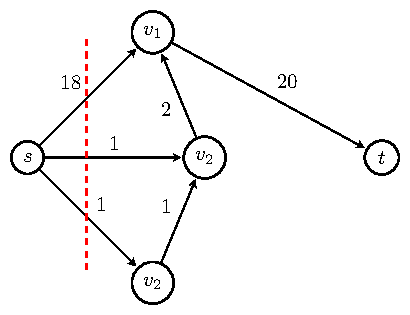
\includegraphics{prueba.pdf}
\end{figure}

\begin{mybox}{titulo}
  Algo
\end{mybox}
\subsection{State Machine}
\tikzset{
	every picture/.append style={
		execute at begin picture={\deactivatequoting},
		execute at end picture={\activatequoting}
	}
}
\begin{tikzpicture}[font=\sffamily]

% Add the states
\node[state,
text=yellow,
draw=none,
fill=gray!50!black] (s) {Sunny};
\node[state,
right=2cm of s,
text=blue!30!white, 
draw=none, 
fill=gray!50!black] (r) {Rainy};

% Connect the states with arrows
\draw[every loop,
auto=right,
line width=1mm,
>=latex,
draw=orange,
fill=orange]
(s) edge[bend right, auto=left]  node {0.6} (r)
(r) edge[bend right, auto=right] node {0.7} (s)
(s) edge[loop above]             node {0.4} (s)
(r) edge[loop above]             node {0.3} (r);
\end{tikzpicture}

\begin{tikzpicture}[auto,node distance=2.8cm]
\tikzstyle{every state}=[fill=red,draw=none,text=white]

\node[initial,state] (A)                    {$q_a$};
\node[state]         (B) [above right of=A] {$q_b$};
\node[state]         (D) [below right of=A] {$q_d$};
\node[state]         (C) [below right of=B] {$q_c$};
\node[state]         (E) [below of=D]       {$q_e$};

\path (A) edge              node {0,1,L} (B)
edge              node {1,1,R} (C)
(B) edge [loop above] node {1,1,L} (B)
edge              node {0,1,L} (C)
(C) edge              node {0,1,L} (D)
edge [bend left]  node {1,0,R} (E)
(D) edge [loop below] node {1,1,R} (D)
edge              node {0,1,R} (A)
(E) edge [bend left]  node {1,0,R} (A);
\end{tikzpicture}
